% !TEX TS-program = pdflatex
% !TEX encoding = UTF-8 Unicode

\documentclass[preprint]{sigplanconf}

\usepackage{graphicx,listings,fixltx2e,lambda,array,multirow,color}


\begin{document}
\conferenceinfo{PLDI 2011}{June 4--8, 2011, San Jose, CA, USA.}
\copyrightyear{2010}

\preprintfooter{PLDI 2011}
\titlebanner{DRAFT---Do not distribute}

\title{Parakeet: General Purpose GPU Programming with Array Languages} 
% EDIT: old title was a bit wordy, looked gross, and "high level" is redundant if someone even glances at our abstract. 
%  --- General Purpose GPU Programming with High Level ArrayLanguages}

\authorinfo{Anonymous}{Anonymous}{Anonymous}
\lstset{ 
basicstyle=\small\footnotesize\ttfamily, % Standardschrift
numbers=left,                   % where to put the line-numbers
stepnumber=1,                   % the step between two line-numbers. If it's 1 each line 
numbersep=12pt,                  % how far the line-numbers are from the code
showspaces=false,               % show spaces adding particular underscores
showstringspaces=false,         % underline spaces within strings
showtabs=false,                 % show tabs within strings adding particular underscores
tabsize=2,	                % sets default tabsize to 2 spaces
captionpos=b,                   % sets the caption-position to bottom
breaklines=true,                % sets automatic line breaking
breakatwhitespace=false,        % sets if automatic breaks should only happen at whitespace
keywordstyle=\color{black}\bf,
morekeywords={til,sum,sqrt,all, min, each, where, while,+,*,-,avg},            % if you want to add more keywords to the set
moredelim=[is][\itshape]{/*}{*/},
linewidth={\textwidth},
xleftmargin=20pt,
%framexleftmargin=17pt,
%framexrightmargin=5pt,
%framexbottommargin=4pt,
}

% define some useful commands to use in language specification 
\newcommand{\WITH}{\impfnt{with}}
\newcommand{\VALUES}{\impfnt{values}}
\newcommand{\MAP}{\impfnt{map}}
\newcommand{\REDUCE}{\impfnt{reduce}}
\newcommand{\ALLPAIRS}{\impfnt{allpairs}}
\newcommand{\CAST}{\impfnt{cast}}
\newcommand{\APPLY}{\impfnt{apply}}
\newcommand{\INDEX}{\impfnt{index}}
\newcommand{\SCAN}{\impfnt{scan}}
\newcommand{\THREADIDX}{\impfnt{threadIdx}}
\newcommand{\BLOCKIDX}{\impfnt{blockIdx}}
\newcommand{\BLOCKDIM}{\impfnt{blockDim}}
\newcommand{\GRIDDIM}{\impfnt{gridDim}}
\newcommand{\VEC}{\impfnt{vec}}
\newcommand{\concat}{\ensuremath{+\!\!\!\!+\,}}

\setlength\fboxsep{8pt}
\setlength\fboxrule{0.5pt}

\maketitle

\begin{abstract}
Contemporary GPUs offer staggering performance potential, which has
led to an explosion in recent work on enabling the execution of
general-purpose programs on GPUs. Despite various advances in making
general-purpose GPU programming easier, the two commonly used
frameworks (NVIDIA's CUDA and OpenCL) are cumbersome and require
detailed architectural knowledge on the part of the programmer to
fully harness this performance potential.

The potential performance advantage over contemporary CPUs that GPUs
offer is due in large part to their having been heavily optimized for
data parallel workloads.  Array-oriented programming--which encourages
the use of data parallel array operators (e.g.\ map, reduce, and
scan), and de-emphasizes the importance of explicit loops--is thus a
natural model for high level programming of GPUs.

We present Parakeet, an intelligent runtime for executing high level
array-oriented programs on GPUs.  The heart of Parakeet is an
interpreter, which upon reaching an array operator synthesizes and
executes a GPU program to implement that operator. Parakeet takes
advantage of runtime information both to choose between different
possible implementations of a GPU program and to set execution
parameters which greatly impact performance. Data is moved transparently
to and from the GPU, and garbage collected when no longer needed. 

We evaluate our system on two standard benchmarks: Black-Scholes
option pricing, and K-Means clustering.  We compare high level
array-oriented implementations to hand-written tuned GPU versions from
the CUDA SDK and the Rodinia GPU benchmark suite. Despite having orders of
magnitude less code, the high level versions perform competitively when executed
by Parakeet.
\end{abstract}

\section{Introduction}
\label{Intro}

Contemporary GPUs boast massive performance potential--in some cases orders of
magnitude higher performance per dollar than that of CPUs--and most desktop
systems today come with graphics processors.  This has led to excellent
recent work on enabling the execution of general-purpose programs on GPUs
(GPGPU)~\cite{Cata10,Main10,Muns10,NvidCU,Sven08,Tard06}. Unfortunately, the two
widely used GPGPU frameworks--NVIDIA's CUDA \cite{NvidCU} and OpenCL
\cite{Muns10}--require the programmer to use extensive knowledge of low level
architectural details in order to fully harness the performance potential.

% Enable programmers to write GPGPU programs in productivity language
Our goal is to lower the barrier to GPGPU programming by allowing programmers to
write in high level array languages that are transparently compiled into
efficient GPU programs. By ``array language'' we mean any language equipped
with:
\begin{enumerate}
\item First-class array values.
\item Succinct syntax for array creation/transformation.
\item Idiomatic preference for bulk array operations instead of explicit loops
(``collection-oriented''~\cite{Sip91} programming).
\end{enumerate}

% Existing Array languages 
The prototypical array language is APL~\cite{Iverson62}, which allows for
extremely terse loop-free specification of algorithms. More commonly used array 
languages include Matlab~\cite{Moler80} (the lingua franca of signal processing
and machine learning research) as well as Python's NumPy~\cite{Oliphant07}
extensions. 


% Heart of Parakeet - an interpreter for our high level IL w/ array ops
In this paper, we present Parakeet, an intelligent runtime for executing high
level array programs on GPUs. Parakeet dynamically specializes user functions 
into a typed intermediate language and transparently executes array operations
on the GPU by synthesizing and launching GPU kernels.


% Q front-end, agnosticism
We have implemented our first Parakeet front end for Q \cite{Borr08}, a
descendant of APL that is widely used in financial computing. 
Q is a nearly ``pure'' array language--its idiomatic style makes sparser use of
loops than even Matlab or NumPy--and is thus a natural first choice.
We are also currently working on front ends for both Matlab and Python.

% Performance
We evaluate Parakeet on two standard benchmark programs: Black-Scholes option
pricing and K-Means clustering.  We compare Q implementations of these
benchmarks run by Parakeet to hand-written, tuned GPU and CPU implementations
from the Rodinia \cite{Che09} and Parsec \cite{Bien08} benchmark suites and the
NVIDIA CUDA SDK \cite{NvidSD}.  Despite the Q implementations requiring orders
of magnitude fewer lines of code, our system delivers competitive performance.

% Bullet-point, drive-home contributions
The main contributions of this paper are the following:

\begin{itemize}
\item A working system in which programmers can write complex, high level code
that is automatically parallelized into efficient GPU programs.
\item A dynamic specialization algorithm that translates a significant subset of
higher-order programs into efficient (unboxed, function-free) GPU code.
\item A low-level intermediate language called \textit{Imp} that captures the
notion of shapely computation \cite{Jay97} necessary in the absence of dynamic
memory allocation.
\item Evidence that dynamically compiling GPU programs can significantly
improve performance by taking advantage of runtime information to
tailor code and execution.
\end{itemize}

\begin{figure*}[t!bh]
\begin{center}
\leavevmode
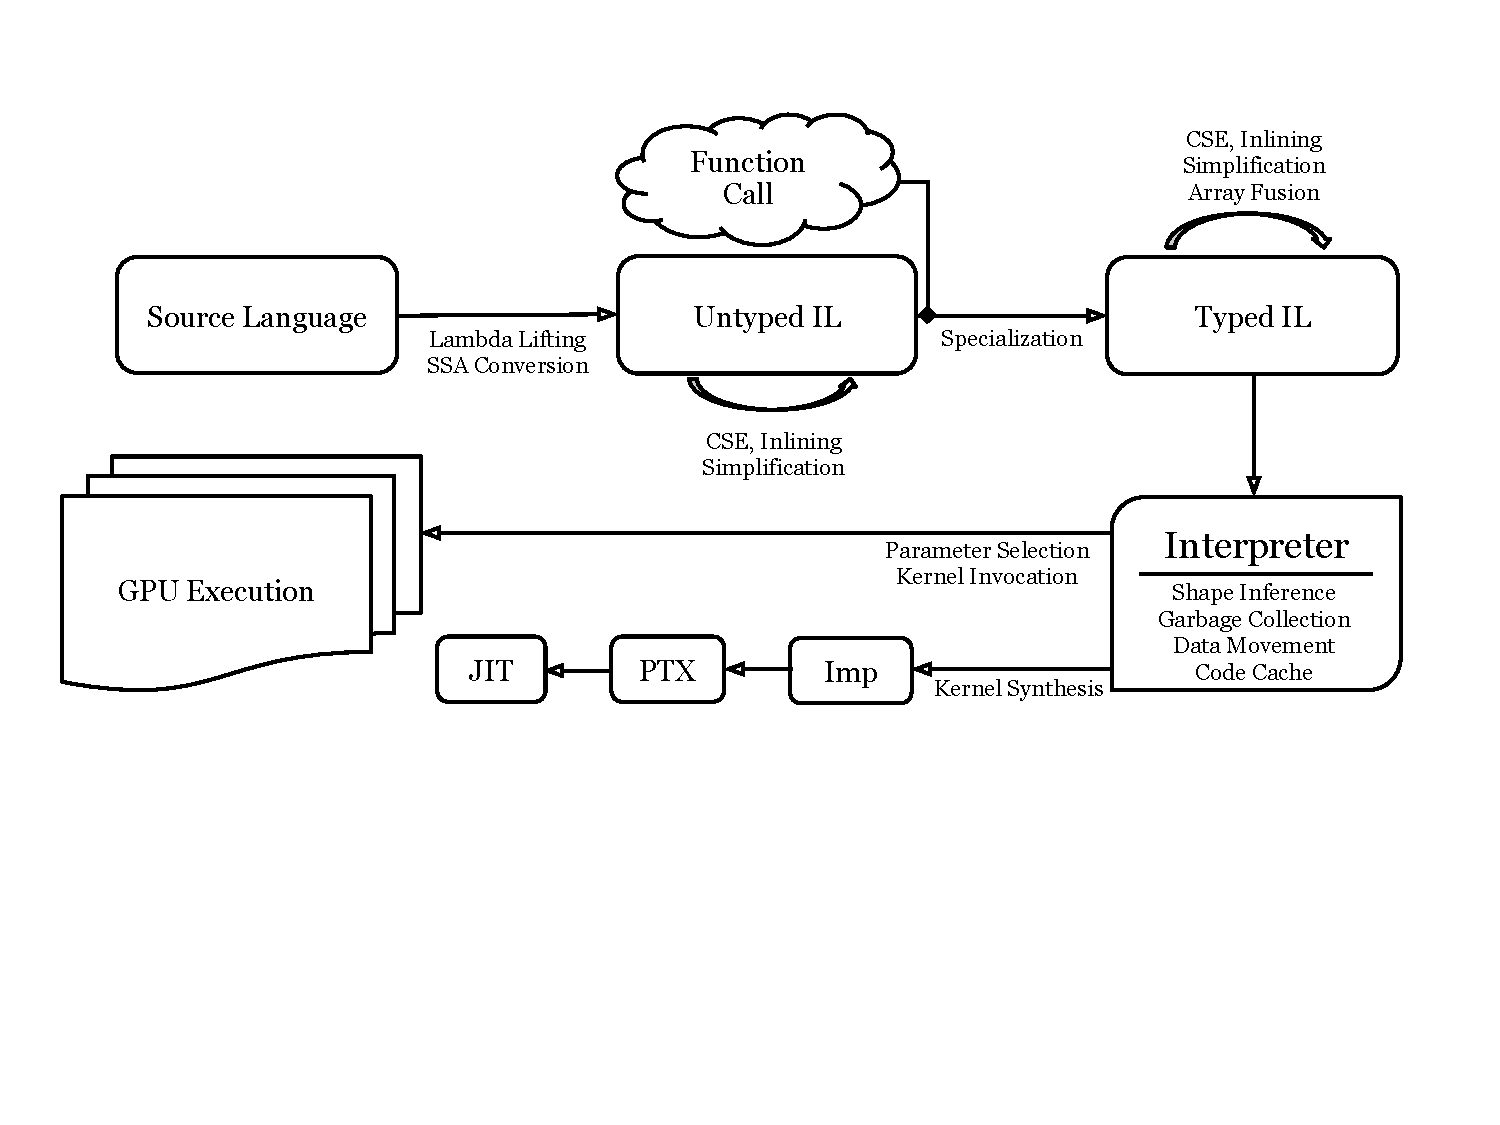
\includegraphics[scale=0.6, trim=10pt 180pt 10pt 120pt]{Pipeline.pdf}
\end{center}
\caption{Overview of Parakeet}
\label{fig:overview}
\end{figure*}
\section{Overview}


%Overview
The pipeline of the execution of a program (shown in Figure
\ref{fig:overview}) begins in the standard interpreter of the source array
language.  The Parakeet framework is attached to the source language's
interpreter as a module, allowing the user to use all of the language's normal
tools and support libraries.  The core of the Parakeet framework its internal
typed intermediate langauge and an interpreter provided for that language. This
IL includes data parallel array operators such as \textbf{map},
\textbf{reduce}, and \textbf{scan} that translate well into efficient data
parallel GPU programs (a full table of the supported operators
can be found in Figure \ref{ArrayOps}).

Execution of a program proceeds in the source language's interpreter, with
Parakeet intercepting function calls.  The source of these functions is then
translated into an untyped intermediate representation. At this step,
various standard compiler optimizations are applied such as common subexpression
elimination.

The function body is then type specialized according to its argument
types.  Further standard optimizations are performed at this stage, as well as
an optimization we call \emph{array operator fusion}.  Here, nested array
operators are fused according to various rewriting rules into fewer operators.
This fusion step, as we will see, is extremely beneficial to the final GPU
program's performance, as it eliminates temporaries and allows for more
efficient use of GPU memory bandwidth.

The Parakeet interpreter then interprets the typed IL function.  When
Parakeet reaches an array operator node in the code tree, it employs a simple
cost-based heuristic (which includes things such as data size and memory
transfer costs) to decide whether to execute that array operator on the GPU or
CPU.  Some code simply cannot be efficiently translated into GPU programs
(such as that which performs I/O or modifies global state), and such code is
kept on the CPU. In the case where Parakeet executes the operator on the CPU,
the operator is either translated into an IL implementation and then further
interpreted by Parakeet, or executed by the source language's interpreter
itself.

If an array operator's computation is deemed a good candidate for GPU
execution, Parakeet flattens all computation nested within that operator
into sequential loops.  This payload is then inlined into a GPU
program skeleton that implements that operator.  For example, in the case of a
\textbf{map}, Parakeet provides a GPU skeleton that implements the pattern of
applying some function to all elements of an array.  The
flattened payload computation of the \textbf{map} is inlined into this
skeleton, and a complete GPU program is synthesized.

To execute the GPU program, Parakeet first copies any of its inputs
that aren't already present on the graphics card to the GPU's memory.  The GPU
program is then executed, with its output lazily brought back to the CPU either
when it is needed or when Parakeet's GPU garbage collector reclaims its space.

\section{GPU Hardware}
To set the stage and motivate the design choices of Parakeet, we first discuss
some important features of modern GPU hardware.  A GPU consists of an array
of tens of multiprocessors.  Within these multiprocessors are various
resources such as local memories and instruction issue units that are shared
among its simple cores. Since the issue units are shared, the threads running
on a single multiprocessor execute instructions in lockstep--hence the name
Single Instruction Multiple Thread (SIMT) for the execution model.  The typical
pattern is to issue a short program to be executed in parallel by thousands
of lightweight threads that run on these hundreds of simple cores, each
operating on different subsets of some input data.  With all these cores, a
typical graphics card has a peak throughput of many hundreds of GLOP/s--an
order of magnitude more than typical high end CPUs at a fraction of the cost.

SIMT differs from the more common Single Instruction Multiple Data (SIMD) model
in that branching instructions are allowed whose branch conditions aren't
uniformly met among threads within a single multiprocessor, allowing colocated
threads to execute divergent code paths.  This improves the ease of programming
a GPU, but divergent branching incurs a very expensive performance penalty as
each thread effectively execute no-ops along the irrelevent code paths.  This
illustrates a common point in GPGPU programming: the hardware allows for
somewhat expressive programming styles, but failure to match what the hardware
actually does well results in very inefficient execution.

Graphics cards have very high peak memory bandwidth--well over 100GB/sec is
common.  However, in order to achieve this high bandwidth (which is essential
to achieving peak performance), nearby threads must access memory in
particular, regular patterns.  Random memory access can be over an order of
magnitude slower than linear stride access.  To alleviate some of this
performance bottleneck, the GPU also provides several other memory spaces with
varying performance characteristics and prefferred access patterns.  These
memory spaces include some read-only cached space (called \emph{texture} and
\emph{constant} memory) and some programmer-managed multiprocessor-local fast
memory called \emph{shared memory}.  Efficient manual use of these memory spaces
can be quite cumbersome, but is also essential to good performance for many
workloads.

\subsection{Limitations Imposed by GPUs}
\label{GPULimitations}
GPUs are able to achieve their specialized high performance because they have
been optimized for particular workloads--viz.~workloads that exhibit \emph{data
parallelism}.  Data parallelism is widely found in typical graphics applications
that perform simple operations on large amounts of pixel or triangle data, and
so is a natural choice for graphics accelerators.  However, this optimization
carries with it various restrictions on the types of code and programming models
that naturally fit the GPU architecture:

\begin{itemize}
\item \textbf{Flat, unboxed data representation}. GPU hardware is optimized to
utilize memory in highly structured access patterns (so-called "coalescing"). 
The use of boxed or indirectly accessed data leads to unstructured memory access
and results in severe performance degradation.

\item \textbf{No polymorphism}. GPUs generally share instruction dispatch units
between many concurrently executing threads. When a group of threads
``diverge'', meaning that they take different branches through a program, their
execution must be serialized. Thus it is important to eliminate as many sources
of runtime uncertainty as possible. In particular, type-tag dispatch commonly
used to implement polymorphic operations would incur unacceptable costs if
translated naively to the GPU.

\item \textbf {No function pointers}. Most GPUs (excluding the recently released
NVIDIA Fermi architecture) do not support the use of indirect jumps or function
pointers. In fact, a common implementation strategy for GPU function calls is
exhaustive inlining. Even in the case where function pointers are theoretically
supported, they require every possible function to be transferred to the GPU and
incur overhead due to potentially unpredictable branching. 

\item \textbf{No global communication}. Synchronization in a GPU computation is
limited to local neighborhoods of threads. Various schemes have been devised for
achieving global synchronization between all executing threads~\cite{feng10},
but these schemes are all either slow or unsafe. This implies that the use of
shared mutable state is a large hindrance to effective utilization of GPU
resources.

\item \textbf{All data must be preallocated}. The current generation of GPUs
lack any mechanism for dynamically allocating memory. Any heap space required by
a GPU computation (for output or temporary values) must be allocated
beforehand. 
\end{itemize}

With these constraints in mind, we turn to our design of efficient high level
abstractions to fit them.

\section{Array Language Programming with Q}
\label{Q}
Array programming languages, as mentioned in Section \ref{Intro}, include
native support for array creation and manipulation via bulk array operators.
These array operators, such as \textbf{map}, typically have natural data
parallel implementations which plays well to the strengths of GPUs.  A key
contribution of Parakeet is to provide a compiler framework that capitalizes on
this strength while respecting the constraints necessary to maintain good
performance.

While we emphasize that the Parakeet framework is built to be agnostic to source
array language, we chose to implement its first front end for Q, a high-level,
sequential array programming language from the APL family \cite{Borr08}.
Q is dynamically typed, and the standard proprietary implementation is
interpreted. Q is a natural choice for Parakeet, since idiomatic Q code uses
native array types and a rich set of array operators and higher-order
data parallel function modifiers that map well onto the Parakeet array
operators. Q is also a fully-featured language, with a large library of built-in
functions, and has a large user base in financial computing. Since our
focus is the Parakeet runtime, we omit many details of the Q language and only
present the salient features so as to illustrate the level of programming
and Q's support for array operators.

\subsection{K-Means Clustering Example}
\begin{figure}[h!]
\begin{lstlisting}
calc_centroid:{[X;a;i] avg X[where a = i]}
calc_centroids:{[X;a;k]
  calc_centroid[X;a] each til k}

dist:{[x;y] sqrt sum (x-y) * (x-y)}
minidx:{[x] x ? min x}

kmeans:{[X;k;a]
  C: calc_centroids[X;a;k];
  converged: 0b;
  while[not converged;
    lastAssignment: a;
    D: X dist/:\: C;
    a: minidx each D;
    C: calc_centroids[X;a;k];
    converged: all lastAssignment = a];
  C}
\end{lstlisting}
\caption{K-Means Clustering implemented in Q}
\label{QKMeans}
\end{figure}

We illustrate the relevant features of array programming in Q with an example:
an implementation of K-Means clustering, a widely used unsupervised
clustering algorithm \cite{MacQ67}.  In Figure \ref{QKMeans}, we see an
implementation of K-Means in Q.  Five functions are defined using Q's bracket
notation for surrounding function bodies and the colon operator for assignment.
For example, the
\texttt{calc\_centroid} function on line 1 takes three parameters
\texttt{X}, \texttt{a}, and \texttt{i} (used as the input data matrix, the
current assignment vector, and the scalar index of the centroid to calculate,
respectively), and calculates that cluster's centroid.

In this function, we illustrate various aspects of the array-oriented nature of
Q. First, Q allows implicit mappings of functions elementwise across
vectors--for example, to test elementwise equality between the assignment
vector \texttt{a} and the index \texttt{i}, we simply write \texttt{a = i}.  In
addition, this showcases Q's support for \emph{scalar promotion}.  In the
statement \texttt{a = i}, \texttt{a} is a vector of integers while \texttt{i} is
a scalar integer.  Semantically, Q implicitly promotes \texttt{i} to be a vector
of the value of \texttt{i} repeated a number of times equal to the length of
\texttt{a} and performs the elementwise equality between these two vectors.

We then generate the list of indices we want by applying the built-in
\texttt{where} operator to the result of this test, and index into the data
matrix \texttt{X} to get the list of data points in the centroid. The result of
this indexing is itself a 2-D matrix which contains the list of data points
belonging to the \texttt{i}-th cluster. Finally, the built-in \texttt{avg}
function--a reduction operator--gets applied to this 2-D list. Thus we see that
reductions and other built-in array operators can be applied to arrays of any
arity.  Further array built-ins used in K-Means include \texttt{sum},
\texttt{min}, and the find operator (denoted by `\texttt{?}').

In this algorithm we also see a number of higher-order data-parallel function
modifier keywords, which in Q are called \emph{adverbs}.  For example, the
\texttt{each} keyword modifies a function by applying it elementwise to its
argument.  In the \texttt{calc\_centroids} function, we calculate each cluster's
new centroid
by using \texttt{each} to apply the \texttt{calc\_centroid} function to a
list of integers from \texttt{0} to \texttt{k-1}.  The other adverb used in
K-Means is what we call \emph{all-pairs}, written `\texttt{/:\char`\\:}'.
(Technically all-pairs is a combination of two adverbs in Q: each-left and
each-right.) All-pairs modifies a binary function and applies it to each
pairs of elements from two input arrays.  We use all-pairs to apply the
\texttt{dist} function to each pair of data point and centroid to calculate all
the needed distances for reassigning the centroids.

We see that array programming languages are both expressive and compact.  While
the CUDA implementation of K-Means in the Rodinia benchmark suite is hundreds of
lines of code long, our Q version is only 17 and could be even more compact.
Now we turn to how we compile array languages to efficient GPU programs.

\section{Typed Intermediate Language}
On first glance, there is a significant mismatch between the highly dynamic
expressiveness of an array language like Q and the limitations imposed by GPU
hardware discussed in Section \ref{GPULimitations}. Indeed, the Parakeet
intermediate language must serve as a compromise between two competing tensions.
First, in order to translate array programs into efficient GPU code it is
necessary for the compiler to eliminate as much abstraction as possible. On the
other hand, we must be careful not to make our program representation overly
concrete with regard to evaluation order (which would eliminate opportunities
for parallelism).

In deference to the above-mentioned GPU hardware restrictions we disallow from
our intermediate language:

\begin{itemize}
\item Polymorphism of all kinds
\item Recursion
\item User-specified higher-order functions
\item Compound data types other than arrays
\end{itemize}

These restrictions are not necessarily as severe as they initially seem, since
the programmer's code is specialized and rewritten into this restricted form
without their awareness.  This is simply the internal format Parakeet uses in
order to generate efficient GPU back end code. We explain in greater detail the
specialization algorithm later on in this paper.

Our intermediate language is shown in Figure \ref{ILandType}. The parallelism
abstraction we prefer to maintain is the use of the higher-order array operators
$\MAP$, $\REDUCE$, and $\SCAN$. The higher-order array operators
form a carefully confined higher-order subset of our otherwise first-order
language and thus we elevate them to primitive syntax. These operators are
important since they are the only constructs in our language that we attempt to
parallelize automatically through GPU code synthesis.

This isn't to say these are the only constructs executed in parallel on the
GPU. The simple array operators such as \textbf{sort} (a full list can be found
in Figure \ref{ArrayOps}) are executed in parallel on the GPU as well. They
simply aren't higher-order, and thus are implemented via a fixed parallel
standard library.

We take inspiration from \cite{Bol09} and allow functions to both accept and
return multiple values. This feature simplifies the specification of certain
optimizations and naturally models the simultaneous creation of multiple values
on the GPU. By convention we will write $\overline{\tau_m}$ to denote a sequence
of $m$ simple types, $\overline{v_n}$ for a sequence  of $n$ values, etc.. A
single element is equivalent to a sequence of length 1 and sequences may be
concatenated via juxtaposition, such that $\tau, \overline{\tau_n} =
\overline{\tau_{m+1}}$.

\begin{figure}
  \begin{tabular}{| m{0.01cm}m{1.5cm}m{0.1cm}m{0.2cm}p{4.5cm} |}
  \hline
  & & & &\\
   \multicolumn{5}{|l|}{\textbf{Intermediate Language Syntax}}  \\[4pt]
  & program & $p$ &  $\bnfdef$   &  $d_1 \cdots d_n $ \\[4pt]
  & definition & $d$ & $\bnfdef$ & $f_i(\overline{x_m} : \overline{\tau_m}) \rightarrow (\overline{y_n} : \overline{\tau_n}) =s^{\small{+}}$ \\[4pt]
  & statement  & $s$ & $\bnfdef$ & $\overline{x_m} : \overline{\rho_m} = e $\\[2pt]
  &            &     & $\sep$    & $\IF \;v\; \THEN \;s^*\; \ELSE \;s^*$ \\[2pt]
  &            &     & $\sep$    & $\WHILE \;e\; \DO \;s^+\;  $ \\[4pt]
  & expression & $e$ & $\bnfdef$ & $ v_{f}(v_1, \ldots, v_m)$ \\[2pt]
  &            &     & $\sep$    & $\textrm{values} (\overline{v_m})$ \\[2pt]
  &            &     & $\sep$    & $\textrm{cast} \; (v, \tau)$ \\[2pt] 
  &            &     & $\sep$    & $\MAP_m (v_{f},\overline{v_m})$ \\[2pt]
  &            &     & $\sep$    & $\REDUCE_m (v_{f}, v_{g}, v_{init}, \overline{v_m})$ \\[2pt]
  &            &     & $\sep$    & $\SCAN_m (v_{f}, v_{g}, v_{init}, \overline{v_m})$ \\[4pt]
  & value      & $v$ & $\bnfdef$ & numeric constant\\[2pt]
  &            &     & $\sep$    &  $x$  \quad \small{(data variable)} \\[2pt]
  &            &     & $\sep$    &  $f$  \quad \small{(function label)} \\[2pt]
  &            &     & $\sep$    &  $\oplus$ \quad \small{(scalar operator)} \\[2pt]
  &            &     & $\sep$    &  $a$ \quad \small{(simple array operator)}
\\[4pt]
  & & & &\\
  \multicolumn{5}{|l|}{\textbf{Type System}} \\[4pt]
  & data     & $\tau$    & $\bnfdef$ & $int \sep float \sep \mathbf{vec} \; \tau   $ \\[4pt]
  & closures        & $\rho$  & $\bnfdef$ & $\{f_i, \overline{\tau_{c}} \} \Rightarrow \overline{\tau_m} \rightarrow \overline{\tau_n}$\\[2pt]
  &                 &           & $\sep$    & $\tau$ \\[4pt]
  & higher-order    & $\theta$  & $\bnfdef$ & $\overline{\rho_m} \rightarrow
\overline{\rho_n} $ \\[4pt]
  & & & &\\
  \hline
  \end{tabular}\\[4pt]
\caption{Intermediate Language and Type System}
\label{ILandType}
\end{figure}

Scalar operators include the usual boolean operations as well as scalar and
floating point arithmetic operators and functions. Examples of simple array
operators include indexing, replication, and inspecting an array's shape.

Salient features of our intermediate language include:
\begin{itemize}
\item In order for higher-order functions to be translated into the Parakeet IL,
it must be possible to specialize away all higher-order arguments. There
are situations where exhaustive specialization is not possible (e.g., combinator
libraries); in these cases, we revert to the source language's interpreter for
execution. This illustrates an important point: since Parakeet augments (but
does not replace) the interpreter of the source language, we are free to
disallow problematic language constructs from Parakeet.

\item It is important to note that we can still represent function values
within our intermediate language (which are created by partial application of
top-level functions). However, since user functions cannot themselves accept
other functions as arguments, the only purpose of function values is to
parameterize the $\MAP$, $\SCAN$, and $\REDUCE$ higher-order primitives.

\item It is also worth highlighting the curious nature of the type we assign to
function values:
$ \{ f_i, \overline{\tau_{c}} \} \Rightarrow \overline{\tau_m} \rightarrow
\overline{\tau_n}$.  The terms occurring before the double arrow ($\{f_i,
\overline{\tau_{c}} \}$) represent both the function label of a closure and the
types of partially applied function arguments. We attach this information to a
closure's type to facilitate efficient passing of closure arguments to the GPU
and avoid any actual indirection which might otherwise be associated with
function invocation. The need to statically determine a function label for any
closure places a serious restriction on which programs Parakeet can compile. We
must reject any code wherein one of multiple functions may be executed at a
program point, depending on some dynamic condition.
\end{itemize}

\begin{figure}
\begin{center}
\begin{tabular}{|p{2.25cm}|p{5.5cm}|}
\hline
\multicolumn{2}{|c|}{\textbf{Higher-Order Array Operators}}\\[4pt] \hline
\textbf{Array Operator} & \textbf{Meaning}\\[4pt] \hline
\textbf{map}($f$,$x$) & Apply function $f$ to all elements of $x$\\[4pt] \hline
\textbf{reduce}($f$,$init$,$x$) & Return result of inserting binary $f$ \\
& between all elements of $x$ prefixed by $init$\\[4pt] \hline
\textbf{scan}($f$,$init$,$x$) & Return running application of $f$ to $init$ \\
& and each element of $x$\\[4pt] \hline
\end{tabular}
\\[12pt]
\begin{tabular}{|p{2.25cm}|p{5.5cm}|}
\hline
\multicolumn{2}{|c|}{\textbf{Simple Array Operators}}\\[4pt] \hline
\textbf{Array Operator} & \textbf{Meaning}\\[4pt] \hline
\textbf{sort}($x$) & Return a sorted version of $x$\\[4pt] \hline
\textbf{find}($x$,$i$) & Return index of first occurence of $i$ in
$x$\\[4pt] \hline
\textbf{where}($x$) & Return an array of indices where $x$ = 1\\[4pt] \hline
\textbf{index}($x$,$i$) & Return the value of $x$ at index $i$\\[4pt] \hline

% Which other ones do we support and want to list?
\end{tabular}
\caption{Parakeet's Supported Array Operators}
\label{ArrayOps}
\end{center}
\end{figure}

\section{Translation, Specialization, and Optimization}
\label{Compilation}
In this section we describe the various program transformations we perform
before executing a user's function. Some of these transformations (such as
lambda lifting and specialization) are necessary in order to bridge the
abstraction gap between an expressive dynamically typed language and the GPU
hardware. We also demonstrate several optimizations which, while beneficial in
any compiler, are particularly important when targetting a graphics processor.
Seemingly small residual inefficiencies in our intermediate form can later
manifest themselves as the creation of large arrays, needless memory transfers,
or wasteful GPU computations.

To help elucidate the different program transformations performed by Parakeet,
we will show the effect of each stage on a distance function defined in Q,
shown in Figure \ref{QDist}.

\begin{figure}[h!]
    \begin{lstlisting}[numbers=none]
    dist: {[x;y] sqrt sum (x-y) * (x-y)}
    \end{lstlisting}
    \caption{Distance Function in Q}
    \label{QDist}
\end{figure}

\subsection{Lambda Lifting and SSA Conversion } 
The first step in the Parakeet pipeline after a function call has been
intercepted by the Parakeet runtime is a syntax-directed translation from a
language-specific AST into Parakeet's IL. Since type information is not yet
available to specialize user functions, they must be translated into an untyped
form (by setting all type assignments to $\bot$). The translation into
Parakeet's IL maintains a closure environment and a name environment so that
simultaneous lambda lifting and SSA conversion can be performed.

Since we would like to interpret our intermediate language we use a gated SSA
form based on the GSA sub-language of the Program Dependence Web \cite{Ott90}.
Classical SSA cannot be directly executed since the $\phi$-nodes lack
deterministic semantics. Gated SSA overcomes this limitation by using "gates"
which not only merge data flow but also associate predicates with each data flow
branch. Aside from simplifying certain optimizations, these gates also enable us
to execute our code without converting out of SSA.  Figure \ref{UntypedSSADist}
shows the \texttt{dist} function after it has been translated to Untyped SSA.

\begin{figure}[h!]
\fbox{
\begin{tabular}{ m{0.1cm} m{6.7cm} }
  \multicolumn{2}{l}{dist $($ x, y $) \rightarrow  ($ z $) =$} \\
  & t$_1 = \mathrm{x} - \mathrm{y} $        \\
  & t$_2 = \mathrm{x} - \mathrm{y} $        \\
  & t$_3  = \mathrm{t}_1 * \mathrm{t}_2 $   \\
  & t$_4  = $sum$(\mathrm{t}_2) $           \\
  & z $  = \; \mathrm{sqrt}(\mathrm{t}_4)$   \\
\end{tabular}
}
\caption{Untyped Distance Function in SSA form}
\label{UntypedSSADist}
\end{figure}


\subsection{Untyped Optimizations}
Parakeet performs optimizations both before and after type specialization. We
subject the untyped representation to inlining, common subexpression elimination
and simplification (which consists of simultaneous constant propagation and dead
code elimination). This step occurs once for each function, upon its first
interception by Parakeet. It is preferable to eliminate as much code as possible
at this early stage since an untyped function body serves as a template for a
potentially large number of future specializations. The only optimizations we do
not perform on the untyped representation are array fusion rewrites, since these
rely on type annotations to ensure correctness.

In our distance example, untyped optimizations will both remove a redundant
subtraction and inline the definition of the $sum$ function, which expands to a
$\REDUCE$ of addition.
\begin{figure}[h!]
\fbox{
\begin{tabular}{ m{0.1cm} m{6.7cm} }
  \multicolumn{2}{l}{dist $($ x, y $) \rightarrow  ($ z $) =$} \\
  & t$_1 = \mathrm{x} - \mathrm{y} $        \\
  & t$_2  = \mathrm{t}_1 * \mathrm{t}_1 $   \\
  & t$_3  = \REDUCE(+, 0, \mathrm{t}_2) $           \\
  & z $  = \; \mathrm{sqrt}(\mathrm{t}_3)$   \\
\end{tabular}
}
\caption{Distance Function after untyped optimizations}
\end{figure}

\subsection{Specialization}
The purpose of specialization is to eliminate polymorphism, to make manifest
all implicit behavior (such as coercion and scalar promotion), and to assign
simple unboxed types to all data used within a function body. Beyond the
fact that the GPU requires its programs to be statically typed, these goals are
all essential for the efficient execution of user code on the GPU.

The most obvious reason for performing specialization is the need to eliminate
polyvariance.  The specializer generates a different specialized version
of a function for each distinct call string, with all of the function's
variables receiving the appropriate types.  The signature of data is one of our
built-in dynamic value types such as $float$ or $vec~int$.  The signature of
functions is a closure that includes a function tag and a list of data
signatures.  It is important to note that specialization is thus not just on
types, but also on function tags and the types of their associated closure
arguments. This is equivalent to performing defunctionalization (Reynolds) and
then specializing exhaustively on the constant values of closure records. One
caveat here is that non-constant closure values are disallowed.  This prevents
us from having to implement them as large switch statements on the GPU, which
would be very inefficient due to branch divergence.  Finally, only data is
allowed to cross the boundary from our system to the source
language--specialized Parakeet functions remain enclosed in our runtime.

To continue the example, if the \textit{dist} function is called with arguments
of type $vec~ float$ the specializer will then generate the code shown in Figure
\ref{SpecDist}.

\begin{figure}[h!]
\fbox{
  \begin{tabular}{m{0.1cm} m{6.7cm}}
    \multicolumn{2}{l}{dist $($ x $ : vec \; float $, y : $ vec \; float $) $
\rightarrow  ($ z $ : float ) =$}  \\
    & t$_1   = \MAP ( -_{\mathrm{float}}, \mathrm{x}, \mathrm{y})$   \\
    & t$_2   = \MAP (*_{\mathrm{float}}, \mathrm{x}, \mathrm{y})$    \\
    & t$_3 = \REDUCE (+_{\mathrm{float}}, 0, \mathrm{t}_2)$          \\
    & z $  = \; \mathrm{sqrt}(\mathrm{t}_3)$                         \\
  \end{tabular}
}
\caption{Distance Function After Specialization}
\label{SpecDist}
\end{figure}

The actual intermediate language associates type annotations with every binding,
which we elide here for clarity. Note that the polymorphism inherent in math
operations between dynamically typed values has been removed through the use of
statically typed math operators, and implicit \textbf{map}s on vectors (such
as the subtraction between $x$ and $y$) have been expanded and made explicit.


\subsection{Array Operator Fusion}
In addition to standard compiler optimizations (such as constant folding,
function inlining, and common sub-expression elimination), we employ fusion
rules~\cite{Jones01} to combine array operators. Fusion enables us to minimize
kernel launches, boost the computational density of generated kernels, and
avoid the generation of unnecessary array temporaries.

We present the fusion rules used by Parakeet in simplified form, such that
array operators only consume and produce a single value. Our rewrite engine
actually generalizes these rules to accept functions of arbitrary input and
output arities, but we elide the full specification for the sake of clarity.
\\[5pt]
\begin{tabular}{|m{0.001cm} m{0.05cm} p{6.75cm} p{0.05cm} |}
  \hline 
  & &  & \\
  & \multicolumn{2}{l}{\large{Map Fusion} }  &  \\[2.5pt]
  & & $\MAP(g, \MAP(f, x)) \leadsto \MAP(g \circ f, x)$ & \\
  & & & \\
  & \multicolumn{2}{l}{\large{Reduce-Map Fusion} }  & \\[2.5pt]
  & & $\REDUCE(g_r, g_{i}, \MAP(f, x)) \leadsto \REDUCE(g_r \circ f, g_{i} \circ f, x)$ & \\
  & & & \\
  \hline
\end{tabular}\\[4pt]
These transformations are safe if the following conditions hold: 
\begin{enumerate}
\item All the functions involved are referentially transparent.

\item Every output of the predecessor function ($f$) is used by the successor
($g$).

\item The outputs of the predecessor are used \textit{only} by the successor.
\end{enumerate}
The last two conditions are severe since they restricit our optimizer from
rewriting anything but linear chains of produced/consumed temporaries. A large
body of previous work~\cite{Ald01} has demonstrated both the existence of
richer fusion rules and cost-directed strategies for applying those rules in
more general scenarios. Still, despite the simplicity of our approach, we have
observed that many wasteful temporaries in idiomatic array code are removed
by using only the above rules.

In Figure \ref{DistFuse}, we see the resulting optimized and specialized
\texttt{dist} function. The two \textbf{map}s have been fused into the
\textbf{reduce} operator, with a new function $f_1$ generated to perform the
computation of all three original higher-order operators.

\begin{figure}[h!]

\fbox{
  \begin{tabular}{m{0.1cm} m{6.7cm} }
    \multicolumn{2}{l}{$\mathrm{f}_1 ($ acc : $ float $,  x $ : float $, y : $ float $) $ \rightarrow  ($ z $ :  float ) =$} \\
    & t$_1 = x - y $            \\
    & t$_2  = t_1 * t_1 $       \\
    & z $ = $ acc $+$ t$_2$     \\
    &  \\ 
  \multicolumn{2}{l}{$\mathrm{dist} ($ x $ : vec \; float $, y : $ vec \; float
$) $ \rightarrow  ($ z $ : float ) =$} \\
  & t$_3 = \REDUCE (\mathrm{f}_1, 0.0, \mathrm{x}, \mathrm{y})$   \\
  & z $ = \mathrm{sqrt}(\mathrm{t}_3)$  \\
  \end{tabular}
}
\caption{Distance Function After Fusion Optimization}
\label{DistFuse}
\end{figure}

\section{GPU Back End}
Before we discuss our GPU code generation, we first walk through the CUDA
programming model in some detail.  Our GPU back end targets NVIDIA GPUs by
emitting PTX--NVIDIA's GPU pseudoassembly language.  NVIDIA GPUs are typically
programmed using CUDA, a higher level C-like wrapper around PTX.  As we will
see in section \ref{Imp}, we have one additional level of intermediate language
in Parakeet before we emit PTX code.

\subsection{CUDA Programming Model}

In CUDA, a program is organized into {\it kernels} and {\it host} code.
Kernels are sequential code that is typically run by many thousands of
lightweight threads on the GPU.  Host code is the code run on the CPU.
Typically, a host thread on the CPU launches a kernel onto the GPU via a C
function call to the CUDA API.  The host thread waits for results and
potentially launches futher kernels.

\subsubsection{CUDA Kernel Organization}

As is typical for data parallel models, all threads in a CUDA kernel execute
the same program code.  This code is specified in a C function using the CUDA C
API. The kernel's threads are organized into {\it thread blocks}, which are
groups of at most a few hundred threads that can communicate and share local
resources. Threads within a given block are all schedule to run on a single GPU
multiprocessor throughput their lifetime.  Threads within a block can
perform barrier synchronizations with each other, but threads from different
blocks have no efficient way to perform synchronization other than termination.
Thus algorithms that require global synchronization (such as parallel reduction)
must be broken up into multiple kernel launches, each of which incurs a small
fixed performance overhead.

The body of a kernel can be written so as to be generic to the number of
threads and blocks with which it is launched, with the programmer specifying at
runtime how many thread blocks are required and how many threads to launch per
block. This allows the kernel programs to be scalable to different datasizes
without requiring rewrites. The standard idiom is for each thread to
be assigned a small computation to be performed on a small subset of some large
input data set.  The threads are each assigned a unique index in the kernel's
{\it grid} of threads, which is used to determine the data for which they are
responsible.

In order to be efficient, CUDA kernels must be dense.  The kernel is executed
by thousands of threads, and any small inefficiencies are greatly magnified.
Manual loop unrolling and rewriting algorithms to have more work per thread are
usually necessary to obtain performance near the GPU's peak potential.

\subsubsection{CUDA Memory Management}

The graphics card has its own memory and GPU kernels cannot access data stored
in the CPU's RAM.  Data must be manually copied back and forth between the CPU
and GPU memory spaces by the CUDA programmer.  This data transfer is roughly
two orders of magnitude slower than memory accesses performed by kernels to the
GPU's memory, and so it is critical for performance that these data transfers
are minimized.  It is also possible and beneficial to overlap memory transfers
with computation.

The main memory space on GPUs is called \emph{global memory} in CUDA.  GPUs have
very high peak memory bandwidth between their processors and global
memory--usually over 100GB/s. This is made possible because the hardware groups
adjacent memory accesses by adjacent threads in a block into single \emph{memory
transactions}. If adjacent threads access misaligned or scattered memory
addresses in a single cycle, these accesses all get serialized, greatly reducing
memory bandwidth for the kernel. Thus the programmer must be very careful
regarding access patterns.  Global memory may or may not be cached depending on
the particular card.

Further, the GPU includes various other memory spaces with different
performance characteristics.  There is \emph{constant memory}, which is
read-only and cached, with the cache optimized for 2D spatial locality.  Each
multiprocessor has a small amount of \emph{shared memory} which all threads
running on that multiprocessor can access and use to synchronize.  Shared
memory is much faster to access than global memory, and is often used as a
programmer-managed cache.  Tiling across input data by placing tiles into
shared memory is a typical trick for reducing global memory traffic.  Register
usage must also be managed, as each multiprocessor's cores shares a common
register pool.  Overallocation of registers causes spillover into global
memory, greatly reducing performance.

%\subsection{GPU Memory Management}
%
%When
%Parakeet synthesizes a GPU program, it first determines whether the input and
%output arguments for that program will fit in their entirety in the available
%GPU memory.  Typically, GPUs have around 500MB to 2GB of RAM, and a significant
%portion of this can be taken up by a user's windowing system.  (In our
%experiments, on a card with 896MB of memory, X Windows can consume well over
%600MB on its own during simple office usage.)  If the data does fit, Parakeet
%copies whatever inputs are not already on the GPU to it and allocates storage
%for the output.  If not, Parakeet chunks the data up into manageable portions,
%copying down one section at a time to the GPU, and then transfering the
%partial result back to the CPU to build the complete result.

\subsection{Imp}
\label{Imp}

As mentioned above, we implement our higher-order array operators as skeletons
of code with splice points where the functions they modify get inlined.  Rather
than implement these skeletons directly in PTX/CUDA, Parakeet
provides a second intermediate language that we call Imp (for imperative).  In
order to inline a function into a higher-order skeleton, we first translate the
function body from the higher level IL into Imp before splicing.

Imp some ways just a wrapper of syntactic sugar around
PTX/CUDA--including, e.g.,~aspects of CUDA such as the special index
registers--that simplifies our job of implementing efficient GPU versions of
these operator skeletons. However, Imp does differ from CUDA in some important
respects:

\begin{enumerate}
\item  Arrays are not associated with a particular GPU memory space (global,
texture, constant, etc..), allowing us to compile variants of an Imp kernel
where inputs reside in different memory spaces.

\item Local temporaries can be arrays in addition to scalars. This generalizes
CUDA's use of ``local'' memory for spilled scalar variables.

\item Space requirements of a function call (all outputs and local arrays it
must allocate) can be determined as a function of input sizes. This is necessary
as GPU computations only have access to memory which is allocated before their
launch and cannot ``dynamically'' allocate more memory.  The shape-related
aspects of Imp's syntax are shown in Figure \ref{ImpSyntax}.
\end{enumerate}
Imp kernels are ``shapely'' by construction, meaning they specify their memory
requirements as deterministic functions of input size. This obviates the
need for ad-hoc allocation logic (the bulk of most CUDA host code) or for
auxilliary size inference on higher level code. If a function can be translate
to Imp then we can always determine its memory requirements.

We perform staged synthesis of Imp kernels by parameterizing them with payload
functions. An Imp kernel can be seen as a ``skeleton'' \cite{Cole04} for a
particular implementation strategy of some array operator.

\begin{figure}
\begin{tabular}{| m{0.1cm}m{1.2cm}m{0.1cm}m{0.2cm}p{2cm}p{2.4cm} |}
\hline
& & & & &\\
 \multicolumn{6}{|l|}{\textbf{Imp Shape-Related Language Syntax}} \\[4pt]
& definition        & $d$      & $\bnfdef$ & 
      \multicolumn{2}{l|}{$f(\overline{x_m} : \overline{\tau_m}) \rightarrow
(\overline{y_n} : \overline{\tau_n}, \overline{\sigma_n}) = s^{\small{+}}$}
\\[4pt]
& shape             & $\sigma$ & $\bnfdef$ & $ [] $                                            &  \quad \small{(shape of scalar)}      \\[2pt]
&                   &          & $\sep$    & $ \sigma \concat \sigma $                         &  \quad \small{(concatenate)}      \\[2pt]
&                   &          & $\sep$    & $ [z] $                                           &  \quad \small{(singleton)}   \\[2pt]
&                   &          & $\sep$    & $ \sigma[\mathrm{const} \ldots  \mathrm{const}] $ &  \quad \small{(slice)}       \\[4pt]
& size              & $z$      & $\bnfdef$ & $ \mathrm{dimsize}(x_i, \mathrm{const}) $         &  \quad \small{(input dimension)}   \\[2pt]
&                   &          & $\sep$    & $ \mathrm{rank}(x_i) $                            &  \quad \small{(input rank)}  \\[2pt]
&                   &          & $\sep$    & $ \oplus(\overline{z_m})$
              &  \quad \small{(scalar primitive)}    \\[2pt]
%& statement         & $s$      & $\bnfdef$ & $x : \tau, \sigma = e $ &
%\\[2pt]
%&                   &          & $\sep$    & $\IF \;v\; \THEN \;s^*\; \ELSE
%\;s^*$ &\\[2pt]
%&                   &          & $\sep$    & $\WHILE \;e\; \DO \;s^+\;  $
%&\\[4pt]
%& expression        & $e$      & $\bnfdef$ & $\oplus(\overline{v_m})$ & \\[2pt]
%&                   &          & $\sep$    & $v_{array}[\overline{v_m}]$
%&\\[2pt]
%&                   &          & $\sep$    & $\textrm{cast} \; (v, \tau)$ &
%\\[2pt] 
%&                   &          & $\sep$    & $\textrm{dimsize}(v_{array},
%v_{int}) $ & \\[2pt]
%&                   &          & $\sep$    & $v$ & \\[4pt]
%& value      & $v$ & $\bnfdef$ &  $x$ & \\[2pt]
%&            &     & $\sep$    &   \multicolumn{2}{l|}{numeric constant}
%\\[2pt]
%&            &     & $\sep$    &  $\mathrm{threadIdx.\{x|y|z\}} $ &\\[2pt]
%&            &     & $\sep$    &  $\mathrm{blockIdx.\{x|y|z\}} $ &\\[2pt]
%&            &     & $\sep$    &  $\mathrm{blockDim.\{x|y|z\}} $ &\\[2pt]
%&            &     & $\sep$    &  $\mathrm{gridDim.\{x|y\}}    $ &\\[2pt]
& & & & &\\
\hline
\end{tabular}
\caption{Imp Language Shape-Related Syntax}
\label{ImpSyntax}
\end{figure}

An example of a simplified Imp skeleton for \textbf{map} is shown in Figure
\ref{ImpMap}.

\begin{figure}[h!]
  \begin{lstlisting}[numbers=none]
    
  \end{lstlisting}
  \caption{Imp Map Skeleton}
  \label{ImpMap}
\end{figure}

\section{Evaluation}
\label{Evaluation}

We evaluated Parakeet on two standard benchmark programs: Black-Scholes option
pricing, and K-Means Clustering.  We compare Parakeet against both hand-tuned
CPU and GPU implementations.  For Black-Scholes, the CPU implementation is
taken from the PARSEC \cite{Bien08} benchmark suite--which we used as the basis
of our Q implementation--and the GPU implementation is taken from the CUDA SDK
\cite{NvidSD}.  For K-Means Clustering, we wrote our own Q version in 17 lines
of code.  Both the CPU and GPU benchmark version come from the Rodinia
benchmark suite \cite{Che09}.

Our experimental setup is as follows.  We ran the CPU benchmarks on a machine
with an Intel Nehalem 2.67GHz X5550 4-core CPU with 24GB of RAM.  The
theoretical peak throughput of this machine is 85.12 GFLOP/s, and it has a
theoretical peak memory bandwidth of 32GB/s.  A key metric for comparing CPUs
to GPUs is also performance per dollar.  At a current market rate of roughly
\$983, the Nehalem has a peak of 0.087 GFLOP/s per dollar.

For all GPU benchmarks, we ran the programs on both an NVIDIA GTX2XX and an
NVIDIA GTX460.  The GTX2XX has 240 processor cores with clock speeds of
Y.YY GHz and YMB of memory, with peak execution throughput of Y.YY GFLOP/s and
peak memory bandwidth of Y.YY GB/s.  The GTX460 has 336 processor cores with
clock speeds of 1.35GHz and 1GB of memory, and has a peak execution throughput
of 907 GFLOP/s and a peak memory bandwidth of 115.2 GB/s.  At a current market
price of roughly \$160, the GTX460 has a peak of 5.67 GFLOP/s per dollar--65
times that of the Nehalem.

For our Parakeet benchmarks, the desktop system we used had a BLAH processor
with BLAH specs.

\subsection{Black-Scholes}
Black-Scholes option pricing \cite{Blac73} is a standard benchmark for data
parallel workloads, since it is embarrassingly parallel--the calculation of the
price of a given option doesn't impact that of any other, and the benchmark
consists of simply running thousands of independent threads in parallel for
computing the prices of thousands of options.

We compare our system against the multithreaded OpenMP CPU implementation
from the PARSEC \cite{Bien08} benchmark suite for both 1 and 4 threads.

\subsection{K-Means Clustering}


\section{Related Work}
\label{RelatedWork}
The use of graphics hardware for non-graphical computation has a long history~\cite{Lengyel90}, though convenient frameworks for general purpose GPU programming have only recently emerged.
The first prominent GPU backend for a general purpose language was ``Brook for
GPUs'' \cite{Buck04}. The Brook language extended C with "kernels" and
"streams", exposing a programming model similar to what is now found in CUDA and
OpenCL. 

Microsoft's Accelerator\cite{Tard06} was the first project to use high level
(collection-oriented) language constructs as a basis for GPU execution.
Accelerator is a declarative GPU language embedded in C\# which creates a
directed acyclic graph of LINQ operations--such as filtering, grouping, and
joining--and compiles them to
(pre-CUDA) shader programs. Accelerator's programming model does not support
function abstractions (only expression trees) and its only underlying
parallelism construct is limited to the production of $\MAP$-like kernels. 

Three more recent projects all translate domain specific embedded array
languages to CUDA backends:
\begin{itemize}
\item \textbf{Nikola}~\cite{Main10} is a first-order array-oriented language
embedded within Haskell. Nikola provides a convenient syntax for expressing
single-kernel computations, but requires the programmer to manually coordinate
computations which require multiple kernel launches. Nikola also does not
support partially applied functions and its parallelization scheme, which first
serializes array operators into loops and then parallelizes loop iterations,
seems ill-suited for complex array operations. 

\item \textbf{Accelerate}~\cite{ChakAcc} is also an embedded array language
within Haskell. Unlike Nikola, Accelerate does allow the expression of
computations which span multiple kernel launches. Accelerate also has a much
richer set of array operators (including the higher-order trio $\MAP$,
$\REDUCE$, $\SCAN$). Accelerate, however, does not seem to support closures or
the nesting of array operators. Accelerate's backend is similar to ours in that
they use a simple interpreter whose job is to initiate skeleton-based kernel
compilation, transfer data to and from the GPU, and to perform simple CPU-side
computations.

\item \textbf{Copperhead}~\cite{Cata10} parallelizes a statically typed purely
functional array subset of Python through the dynamic compilation/execution of
CUDA kernels. Copperhead supports nested array computations, and even has a
sophisticated notion of where these computations can be scheduled. In addition
to sequentializing nested array operators within CUDA kernels (as done in
Parakeet), Copperhead can also share the work of a nested computation between
all the threads in CUDA block. Unfortunately, Copperhead does not utilize any
dynamic information (such as size) when making these scheduling decisions and
thus must rely on user annotations. Copperhead's compiler generates kernels
through parameterization of operator-specific C++ template classes. By using C++
as their backend target, Copperhead has been able to easily integrate the Thrust
~\cite{Hobe10} GPGPU library and to offload the bulk of their
code optimizations onto a C++ compiler. Runtime generation of templated C++ can,
however, be a double-edged sword. Copperhead experiences the longest compile
times of any project mentioned here (orders of magnitude longer than the
compiler overhead of Parakeet).
\end{itemize} 
Unlike the three approaches mentioned above, Parakeet does not require its
source language to be purely functional nor statically typed. Being able to
program in a dynamically typed language seems particularly important for array
computations, since static type systems are generally unable to support the
syntactic conveniences which make array programming appealing in the first
place.

\section{Conclusion}
\label{Conclusion}

We have presented Parakeet, an intelligent runtime for executing high level
array-oriented programs on GPUs.  Parakeet alleviates programmers from having
to write code that explicitly manages low level architectural details, pushing
the level of abstraction for GPGPU programming up to the level of productivity
languages.  Parakeet automatically synthesizes GPU programs from data parallel
array operators, transparently running these programs and moving data back and
forth to the GPU's memory and performing GPU memory garbage collection.
Parakeet includes a series of optimizations to generate more efficient GPU
programs, including array operator fusion and the use of shared and texture
memory on the GPU.  Parakeet is a working system, in which complex programs can
be written and executed efficiently.  On two benchmark programs, Parakeet
delivers performance competitive with even hand-tuned CPU and GPU
implementations.

In future work, we hope to support more front ends and back ends.  At the
moment, we are building front ends for both Matlab and Python.  We envision
building a back end for multicore CPUs as well, likely targeting LLVM
\cite{Latt02}.  In addition, we have many ideas on how to take advantage of
dynamicism to produce more efficient code and executions.  These include things
such as iteratively tuning components of hierarchical algorithms, splitting
data inputs to take advantage of more of the texturing hardware, and overlapping
computation with data transfer.  With all of the basic machinery of Parakeet now
in place, we can explore this research space.

\bibliographystyle{acm}
\bibliography{../Parallelism}{}

\end{document}
